\section{Problem}
Når objekters funktionalitet distribueres ud mellem hinanden, vil der opstå høj kobling, og masser af interkonnektivitet.  I et mediator pattern oprettes et separat mediator-objekt, som står for at kontrollere objekters interaktioner med hinanden. 

\section{Løsning}

\begin{figure}[h]
	\centering
	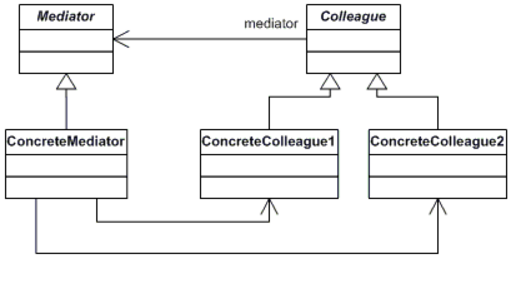
\includegraphics[width=\linewidth]{figs/concrete}
	\caption{Generelt klassediagram om Mediator pattern.}
	\label{fig:concrete}
\end{figure}

Definition og identifikation af deltagende klassers type:

\begin{itemize}
	\item Mediator.
	\begin{itemize}
		\item 	Definerer et interface til kommunikation med “Colleague objekter”.
	\end{itemize}
	\item Concrete mediator.
	\begin{itemize}
		\item 	Implementerer kommunikationsinterfacet, ved at koordinere Colleague objekter.
	\end{itemize}
	\item Colleague klasser.
	\begin{itemize}
		\item Hver colleague klasse kender sit mediator object.
		\item Når colleaguen vil snakke med en anden klasse, kommunikeres der udelukkende gennem mediatoren.
	\end{itemize}
\end{itemize}

Brugen af et mediator pattern begrænser mængden af afledte klasser i et system, i og med mediatoren centraliserer funktionalitet der ellers ville være spredt ud på mange klasser. Ved at pakke objekters interkonnektivitet ind i et mediator pattern, får man samtidig skabt et ekstra abtraktionsniveau der gør funktionalitet mere overskuelig.

\section{Eksempel}
Her følger et eksempel på brugen af Mediator pattern. Kildekoden kan ses på github\footnote{\url{https://github.com/BjornNorgaard/I4SWD/tree/master/MediatorPattern}} I eksempelet vil afledte klasser af typen \textit{Participant} kommunikere indbyrdes. Eksempelet er holdt simpelt idet at klasserne via Mediatoren kun kan sende \textit{strings} til hinanden, men selvfølgelig ville dette kunne ændres til hvad end man har brug for.

\begin{lstlisting}
static void Main(string[] args)
{
	Mediator Chatroom = new Mediator();
	
	Participant Dennis = new Borger("Dennis");
	Participant Joachim = new Borger("Joachim");
	
	Chatroom.Register(Dennis);
	Chatroom.Register(Joachim);
	
	Dennis.Send("Joachim", "Herro Jokke!");
	Joachim.Send("Dennis", "Hello Dennis");
}
\end{lstlisting}

Hele klassediagrammet for programmet kan ses på figur~\ref{fig:mediclass} på side~\pageref{fig:mediclass}. En \textit{Participant} har et Mediator medlem og denne bliver sat med \textit{Chatroom.Register(''Parcipant'');} metoden. Hvorved Mediatoren sætte sig selv som netop denne mediator. Implementering ses her:

\begin{lstlisting}
// you can search for complex class with simple key, i.e. string in this case
protected Dictionary<string, IParticipant> Participants;

public virtual void Register(IParticipant participant)
{
	// checking if participant is already in dictionary
	if (Participants.ContainsValue(participant) == false)
		Participants[participant.Name] = participant;
	
	// adding this mediator object to participant when registering
	participant.Mediator = this;
}
\end{lstlisting}

Det er også i Mediatorens \textit{Register} metode at den indeksere det gældende object af typen IParticipant, i dette tilfælde ved \textit{Name} af typen \textit{string}. 

Når en Participant vil sende en besked skal den bare kende modtagerens navn og kalde sin mediators \textit{Send} metode, som det kan ses herunder:

\begin{lstlisting}
public virtual void Send(string to, string message)
{
	// Name being the "return-address"/Senders name
	Mediator.Send(Name, to, message);
}
\end{lstlisting}

Når Mediatoren så skal videreformidle denne besked skal den blot kalde modtagerens \textit{Receive} funktion.

\begin{lstlisting}
public virtual void Send(string from, string to, string message)
{
	// using dict's key as receiver, no need for actual value/object
	IParticipant participant = Participants[to];
	
	if (participant != null)
		participant.Receive(from, message);
}
\end{lstlisting}

Herefter kan modtageren så gøre med besked hvad den nu skal. I dette eksempel vil den blot lave en udskrift:

\begin{lstlisting}
public virtual void Receive(string from, string message)
{
	Console.WriteLine(from + " to " + Name + ": " + message);
}
\end{lstlisting}

Her følger klassediagrammet for implementering af eksemplet:

\begin{figure}[h]
	\centering
	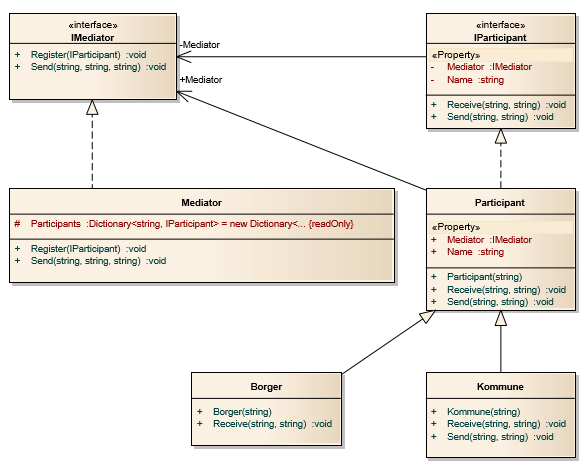
\includegraphics[width=\linewidth]{figs/classdiagram}
	\caption{Klassediagram for vores eksempel på Mediator pattern.}
	\label{fig:mediclass}
\end{figure}

\section{Sammenligning}

\subsection{Publisher-subscriber}
Mediator patternet kan sammenlignes med publisher-subscriber. Begge står for at håndtere kommunikationen mellem to eller flere klasser. Hvor publisher-subscriber blot broadcaster til alle subscribers, så har mediatoren i højere grad funktionalitet til at finde ud af, hvilke "colleague" eller "subscribers" der skal udføres noget på. Wiki har et glimrende eksempel på siden om Mediator\footnote{\url{https://en.wikipedia.org/wiki/Mediator_pattern#Java} - Mediator eksempel i Java}, som viser, at alt efter hvilken kommando der kaldes, så udfører mediatoren noget forskelligt, og kalder metoderne hos de registrerede objekter med forskellige parametre.

\subsection{Konsekvenser}
Mediatoren samler en masse funktionalitet på ét sted, hvilket har den fordel at interaktionen mellem objekter bliver nemmere, men mediatoren får derved større ansvar og bliver mere kompleks. Mediatoren kan derfor hurtigt blive en monolit, som er svær at vedligeholde.

\section{Konklusion}
Ud fra journalen kan det konkluderes, at Mediator pattern er godt at bruge, i tilfælde, hvor der opstår mange forbindelser mellem mange forskellige klasser. Ved hjælp af mediatoren centraliseres referencerne til de forskellige objekter ét sted, og samler kald til mediatoren, i stedet for enkelte klasser. Dog skal der passes på at mediatoren ikke bliver til en monolit, hvis for meget funktionalitet bliver pakket ind i den.

\begin{figure}[h]
	\centering
	
\includegraphics[width=1\linewidth]{figs/topgunn}
	\caption{Figure of awesome}
	\label{fig:topgunn}
\end{figure}

